% Fig. 3.27 -- two order statistics Y_i and Y_j taken together split the
%   support into three stretches, holding i-1, j-i-1 and n-j of the sample.
% Source: mathstatch3.tex lines 5354-5373.  Manuscript geometry kept: the
%   same number line as Fig. 3.24, dividers at x = 3 and x = 7 named y_i and
%   y_j, the counts above the line at x = 1.5, 5 and 8.5, and three dashed
%   arcs under the line spanning 0 to 3, 3 to 7 and 7 to 9.95, labelled with
%   the probability that one sample value falls in that stretch.
%
% Fourth of the series 3.24-3.27; coordinates, divider height, arc depth and
% type size are those of order-stat-min.tex, and the four departures from the
% manuscript picture recorded there apply here unchanged (counts left as bare
% mathematics, y_i and y_j carried at the top of the dividers, arcs drawn as
% cubics of sag 0.40, F_{\sssig X} written F_X).
%
% The middle label is the long one.  At 76.60pt it reaches 1.58 units either
% side of x = 5, so its box clears the box of the left arc's label by 1.00cm
% and that of the right arc's label by 0.68cm, both above the 0.6cm of spec
% 1.3; this is what sets the drawing width of the whole series.  Under the
% manuscript's own layout, with y_i and y_j hanging beneath the axis, it
% would instead have come within 0.05cm of the y_i label.
%
% \DeclareMathSizes{10}{10}{9}{8} raises the math script sizes from the
% default 7pt/5pt.  Native width 249.343pt (drawing range 8.63cm, inside the
% 9.0cm cap of spec 1.3).  A mark of S pt shows at
% S x 0.99626 x <display width> / 249.343 px, so in a topic-figure--wide at the
% 350px phone width
%     10pt text 13.98px, 9pt scripts 12.59px
% and at the 620px desktop width 24.77 / 22.30px.  The smallest marks in the
% picture are the X of F_X and the i and j of y_i and y_j, all at script
% size.
\documentclass[tikz,border=2pt]{standalone}
\usepackage{amsmath}
\usepackage{amssymb}
\usepackage{xcolor}
\usetikzlibrary{arrows.meta}
\DeclareMathSizes{10}{10}{9}{8}

\definecolor{journalink}{HTML}{1F1C18}
\definecolor{journalmuted}{HTML}{8A7F72}
\definecolor{journalaccent}{HTML}{9C2D2D}

\begin{document}
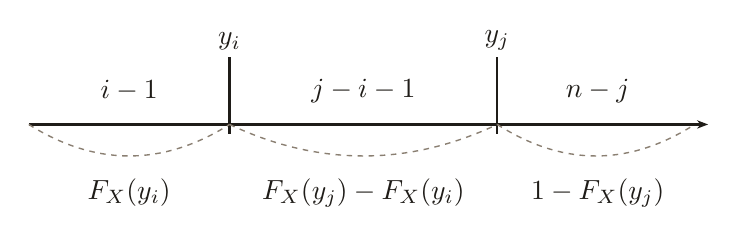
\begin{tikzpicture}[
  x=0.85cm,
  y=1cm,
  every node/.style={font=\normalsize, journalink, inner sep=1pt},
  axis/.style={journalink, line width=0.8pt, -{Stealth[length=4pt]}},
  divider/.style={journalink, line width=0.8pt},
  arc/.style={journalmuted, line width=0.5pt, dash pattern=on 2pt off 2pt}
]
  % ---- the number line -------------------------------------------------
  \draw[axis] (0,0) -- (10.15,0);

  % ---- the cuts at y_i and y_j -----------------------------------------
  \draw[divider] (3,-0.12) -- (3,0.86);
  \node[anchor=south] at (3,0.90) {$y_i$};
  \draw[divider] (7,-0.12) -- (7,0.86);
  \node[anchor=south] at (7,0.90) {$y_j$};

  % ---- how many of the sample lie in each stretch ----------------------
  \node at (1.5,0.43) {$i-1$};
  \node at (5,0.43) {$j-i-1$};
  \node at (8.5,0.43) {$n-j$};

  % ---- the probability of each stretch ---------------------------------
  \draw[arc] (0,0) .. controls (1,-0.5333) and (2,-0.5333) .. (3,0);
  \draw[arc] (3,0) .. controls (4.3333,-0.5333) and (5.6667,-0.5333) .. (7,0);
  \draw[arc] (7,0) .. controls (7.9833,-0.5333) and (8.9667,-0.5333)
    .. (9.95,0);
  \node[anchor=north] at (1.5,-0.65) {$F_X(y_i)$};
  \node[anchor=north] at (5,-0.65) {$F_X(y_j)-F_X(y_i)$};
  \node[anchor=north] at (8.5,-0.65) {$1-F_X(y_j)$};
\end{tikzpicture}
\end{document}
